\documentclass[A4,svgnames,9pt,aspectratio=169]{beamer}

\usepackage[utf8]{inputenc}
\usepackage[T1]{fontenc}
\usepackage[french]{babel}
\usepackage{graphicx}
\usepackage{amsmath,amssymb}
\usepackage{booktabs}
\usepackage{array}
\usepackage{tabularx}
\usepackage{xcolor}
\usepackage{tikz}
\usetikzlibrary{arrows.meta,calc,fit,positioning,shapes.geometric}

\usetheme{inria}
\graphicspath{{figures/}}

\hypersetup{
  colorlinks=true,
  allcolors=rouge_inria,
  pdfauthor={Louis Hauseux, Raphaël Antoine, Philippe Foucher, Pierre Charbonnier, Josiane Zerubia},
  pdftitle={Frangi-graphe et CrackSAM 2},
  pdfsubject={Diagnostic des essais Frangi-similarité avec SAM 2 et feuille de route},
  pdfkeywords={SAM, SAM 2, SAM 3, CrackSAM, Frangi, graph, crack segmentation}
}

\definecolor{success}{HTML}{3C8D5A}
\definecolor{warning}{HTML}{D98200}
\definecolor{failure}{HTML}{C9191E}
\definecolor{inkblue}{HTML}{27348B}
\definecolor{softblue}{HTML}{E9F2F8}
\definecolor{softred}{HTML}{FBEAEC}
\definecolor{softgreen}{HTML}{EAF5EE}
\definecolor{softgray}{HTML}{F1F2F4}

\newcommand{\Frangi}{\textsc{Frangi}}
\newcommand{\SAM}{\textsc{SAM}}
\newcommand{\IoU}{\mathrm{IoU}}
\newcommand{\source}[1]{%
  \par\vfill{\raggedright\fontsize{5.8}{6.6}\selectfont\color{black!58}#1\par}%
}
\newcommand{\statusbadge}[2]{%
  \tikz[baseline=(n.base)]\node[rounded corners=2pt,fill=#1!13,draw=#1!55,
  inner xsep=4pt,inner ysep=1.5pt,text=#1,font=\bfseries\scriptsize] (n) {#2};%
}
\newcommand{\metriccard}[4]{%
  \begin{tikzpicture}
    \node[rounded corners=4pt,draw=#1!50,fill=#1!8,minimum width=3.05cm,
      minimum height=1.35cm,align=center,inner sep=4pt] {%
      {\scriptsize #2}\\[-1pt]
      {\Large\bfseries\color{#1} #3}\\[-1pt]
      {\fontsize{5.8}{6.5}\selectfont\color{black!62} #4}%
    };
  \end{tikzpicture}%
}
\newcommand{\imagepanel}[2]{%
  \begin{minipage}[t]{0.188\textwidth}
    \centering
    {\scriptsize\bfseries #1}\par\vspace{2pt}
    \fcolorbox{black!18}{white}{\includegraphics[width=0.94\linewidth]{#2}}
  \end{minipage}%
}
\newcommand{\litcard}[4]{%
  \begin{tikzpicture}
    \node[rounded corners=4pt,draw=#1!48,fill=#1!7,text width=4.05cm,
      minimum height=1.72cm,align=left,inner sep=6pt] {%
      {\bfseries\color{#1} #2}\hfill{\tiny #3}\\[2pt]
      {\scriptsize #4}%
    };
  \end{tikzpicture}%
}

\title[Frangi-graphe $\times$ CrackSAM 2]{Frangi-graphe $\times$ CrackSAM 2}
\subtitle{Ce qui a été testé, pourquoi le prompt dense échoue, et la suite}
\date[25/07/2026]{25 juillet 2026}
\author[L. \textsc{Hauseux} et al.]{%
  {\small Inria, équipe \textsc{Ayana} : Louis \textsc{Hauseux}, Josiane \textsc{Zerubia}}\\
  {\small Cerema, équipe \textsc{Endsum} : Raphaël \textsc{Antoine}, Philippe \textsc{Foucher}, Pierre \textsc{Charbonnier}}%
}
\institute{Inria, Université Côte d'Azur \quad---\quad Cerema}

\begin{document}

\frame{\titlepage}

\begin{frame}{La question n'est plus \og Frangi améliore-t-il SAM ?\fg{}}
  \centering
  \vspace{0.3cm}
  \begin{tikzpicture}[node distance=0.75cm and 0.75cm,>=Latex]
    \node[rounded corners=6pt,draw=inkblue!55,fill=softblue,
      minimum width=3.2cm,minimum height=2.05cm,align=center] (propose) {
      {\Large\bfseries\color{inkblue} 1. Proposer}\\[3pt]
      \Frangi-graphe\\
      {\scriptsize lignes, orientations, connexions}};
    \node[rounded corners=6pt,draw=warning!60,fill=warning!8,
      minimum width=3.2cm,minimum height=2.05cm,align=center,right=of propose] (verify) {
      {\Large\bfseries\color{warning} 2. Vérifier}\\[3pt]
      Features \SAM\\
      {\scriptsize fissure ou structure trompeuse ?}};
    \node[rounded corners=6pt,draw=success!60,fill=softgreen,
      minimum width=3.2cm,minimum height=2.05cm,align=center,right=of verify] (correct) {
      {\Large\bfseries\color{success} 3. Corriger}\\[3pt]
      Résidu local\\
      {\scriptsize sinon retour exact à la baseline}};
    \draw[->,very thick,inkblue] (propose) -- (verify);
    \draw[->,very thick,warning] (verify) -- (correct);
    \node[below=0.65cm of verify,align=center,text width=11.2cm] {
      \Large\bfseries Une géométrie utile n'est pas encore une décision sémantique.
    };
  \end{tikzpicture}

  \source{Question expérimentale et architecture actives du dépôt, juillet 2026.}
\end{frame}

% -----------------------------------------------------------------------------
\section{De SAM à CrackSAM}
\frame{\sectionpage}

\begin{frame}{SAM : segmenter à partir d'une invite}
  \begin{columns}[T,onlytextwidth]
    \begin{column}{0.58\textwidth}
      \centering
      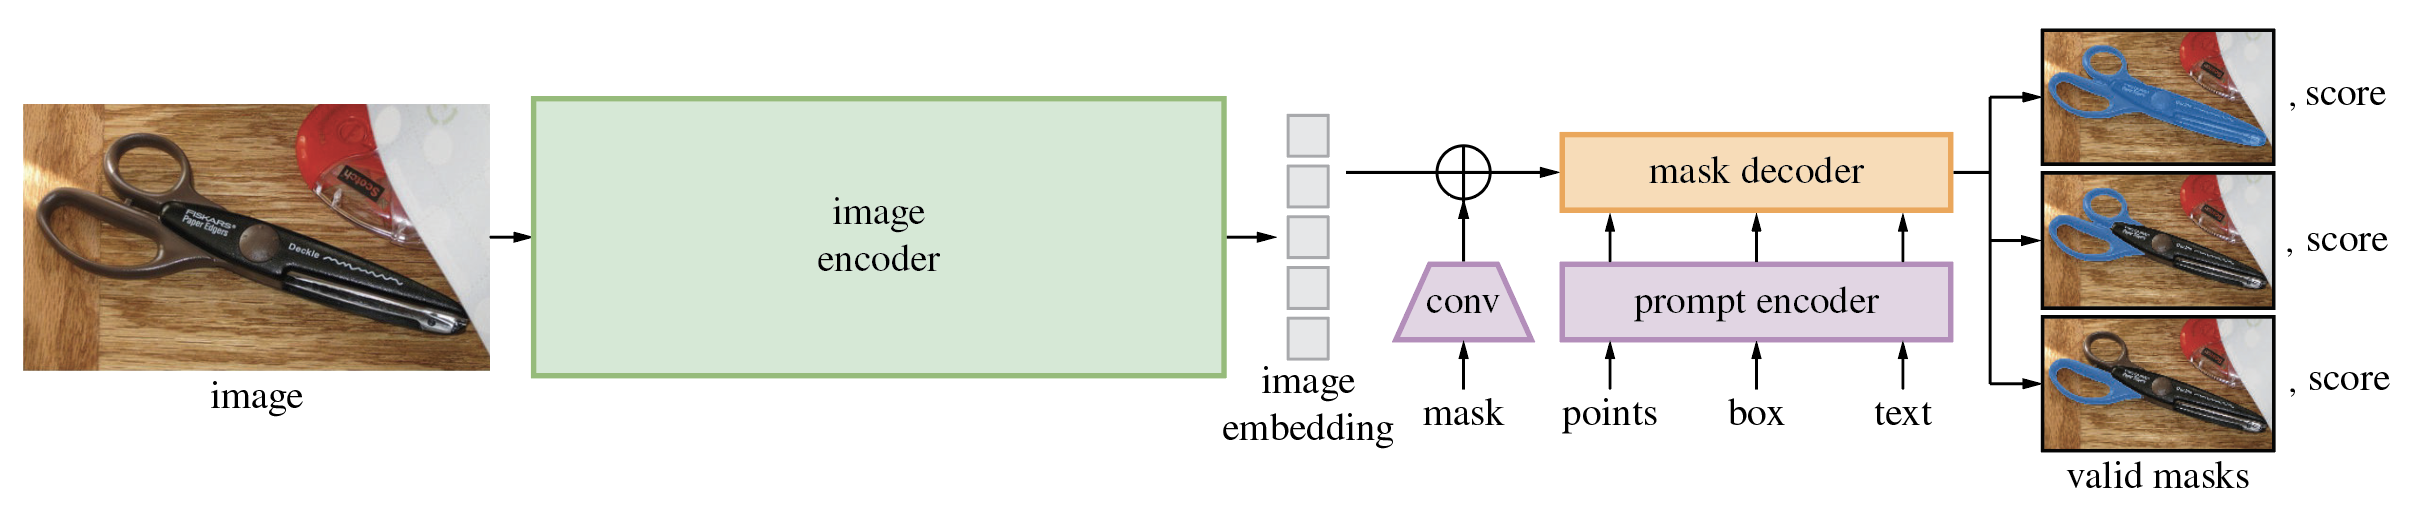
\includegraphics[width=\linewidth,height=0.61\textheight,keepaspectratio]{sam_model_diagram.png}
    \end{column}
    \begin{column}{0.39\textwidth}
      \vspace{0.2cm}
      \begin{tikzpicture}[node distance=0.34cm]
        \node[rounded corners=4pt,draw=inkblue!45,fill=softblue,
          text width=4.25cm,align=left,inner sep=6pt] (enc) {
          \textbf{Encodeur image}\\[-1pt]
          {\scriptsize ViT lourd, calculé une fois}};
        \node[rounded corners=4pt,draw=warning!50,fill=warning!7,
          text width=4.25cm,align=left,inner sep=6pt,below=of enc] (prompt) {
          \textbf{Encodeur d'invites}\\[-1pt]
          {\scriptsize points, boîte, masque}};
        \node[rounded corners=4pt,draw=success!50,fill=softgreen,
          text width=4.25cm,align=left,inner sep=6pt,below=of prompt] (dec) {
          \textbf{Décodeur de masque}\\[-1pt]
          {\scriptsize léger, interactif, ambiguïté possible}};
      \end{tikzpicture}
      \vspace{0.25cm}

      \begin{block}{Le point clé}
        \small SAM apprend une \textbf{interface de segmentation guidée}, pas une classe \og fissure\fg{}.
      \end{block}
    \end{column}
  \end{columns}
  \source{Kirillov et al., \href{https://arxiv.org/abs/2304.02643}{\emph{Segment Anything}}, ICCV 2023. SA-1B : 11 M d'images, 1,1 milliard de masques.}
\end{frame}

\begin{frame}{SAM 2 : même dialogue, backbone et mémoire repensés}
  \centering
  \begin{tikzpicture}[>=Latex,node distance=0.58cm and 0.72cm]
    \node[rounded corners=5pt,draw=inkblue!55,fill=softblue,
      minimum width=2.8cm,minimum height=1.45cm,align=center] (hiera) {
      {\bfseries Hiera}\\{\scriptsize pyramide multi-échelle}};
    \node[rounded corners=5pt,draw=warning!55,fill=warning!8,
      minimum width=2.55cm,minimum height=1.45cm,align=center,right=of hiera] (memory) {
      {\bfseries Mémoire}\\{\scriptsize objets dans le temps}};
    \node[rounded corners=5pt,draw=success!55,fill=softgreen,
      minimum width=2.7cm,minimum height=1.45cm,align=center,right=of memory] (decoder) {
      {\bfseries Décodeur}\\{\scriptsize image ou masklet vidéo}};
    \draw[->,very thick] (hiera) -- (memory);
    \draw[->,very thick] (memory) -- (decoder);
    \node[above=0.45cm of memory,font=\Large\bfseries] {SAM 2};
    \node[below=0.55cm of hiera,rounded corners=4pt,fill=inkblue!7,
      draw=inkblue!35,text width=3cm,align=center,inner sep=5pt] {
      {\scriptsize features haute résolution utiles aux fissures fines}};
    \node[below=0.55cm of memory,rounded corners=4pt,fill=warning!7,
      draw=warning!35,text width=3cm,align=center,inner sep=5pt] {
      {\scriptsize une image est un \og film\fg{} d'une seule frame}};
    \node[below=0.55cm of decoder,rounded corners=4pt,fill=success!7,
      draw=success!35,text width=3cm,align=center,inner sep=5pt] {
      {\scriptsize API points / boîtes / masques conservée}};
  \end{tikzpicture}

  \vspace{0.55cm}
  \begin{columns}[T,onlytextwidth]
    \begin{column}{0.48\textwidth}
      \begin{block}{Selon l'article SAM 2}
        \centering\large Plus précis et \textbf{$6\times$ plus rapide} que SAM en segmentation d'image.
      \end{block}
    \end{column}
    \begin{column}{0.48\textwidth}
      \begin{block}{Dans ce projet}
        \centering\large Hiera-L + LoRA $q/v$ ; mode image sans mémoire temporelle.
      \end{block}
    \end{column}
  \end{columns}
  \source{Ravi et al., \href{https://arxiv.org/abs/2408.00714}{\emph{SAM 2: Segment Anything in Images and Videos}}, 2024. Le dépôt officiel publie aussi les checkpoints SAM 2.1.}
\end{frame}

\begin{frame}{SAM 3 : de l'objet pointé au concept recherché}
  \begin{columns}[T,onlytextwidth]
    \begin{column}{0.50\textwidth}
      \centering
      \begin{tikzpicture}[node distance=0.42cm,>=Latex]
        \node[rounded corners=5pt,draw=black!35,fill=softgray,
          minimum width=4.8cm,minimum height=0.78cm,align=center] (classic) {
          \textbf{Invite visuelle} : point, boîte, masque};
        \node[rounded corners=5pt,draw=inkblue!50,fill=softblue,
          minimum width=4.8cm,minimum height=0.78cm,align=center,below=of classic] (text) {
          \textbf{Concept} : \og fissure de chaussée\fg{}};
        \node[rounded corners=5pt,draw=warning!55,fill=warning!8,
          minimum width=4.8cm,minimum height=0.78cm,align=center,below=of text] (example) {
          \textbf{Exemplaires} : positifs et négatifs};
        \node[rounded corners=6pt,draw=success!55,fill=softgreen,
          minimum width=4.8cm,minimum height=1.1cm,align=center,below=0.55cm of example] (sam3) {
          {\large\bfseries SAM 3}\\[-1pt]
          {\scriptsize détecter + segmenter + suivre toutes les instances}};
        \draw[->,thick] (classic) -- (sam3);
        \draw[->,thick,inkblue] (text) -- (sam3);
        \draw[->,thick,warning] (example) -- (sam3);
      \end{tikzpicture}
    \end{column}
    \begin{column}{0.47\textwidth}
      \statusbadge{inkblue}{Piste parallèle, non testée ici}
      \vspace{0.28cm}
      \begin{itemize}
        \item Détecteur image + tracker à mémoire, backbone partagé.
        \item Tête de \textbf{présence} : reconnaissance séparée de la localisation.
        \item Prompts texte et exemplaires : intéressants pour \textbf{vérifier} une composante Frangi.
      \end{itemize}
      \begin{alertblock}{Ce que SAM 3 ne garantit pas}
        Résolution des fissures fines, connectivité du graphe et robustesse aux ombres restent à mesurer.
      \end{alertblock}
    \end{column}
  \end{columns}
  \source{Carion et al., \href{https://arxiv.org/abs/2511.16719}{\emph{SAM 3: Segment Anything with Concepts}}, ICLR 2026.}
\end{frame}

\begin{frame}{CrackSAM : transformer SAM en segmenter automatique de fissures}
  \begin{columns}[T,onlytextwidth]
    \begin{column}{0.42\textwidth}
      \vspace{0.15cm}
      \begin{block}{Adaptation efficace}
        \centering
        \[
          W = W_0 + BA, \qquad \operatorname{rang}(BA)=r
        \]
        \small LoRA ou adaptateurs ; le socle SAM reste largement gelé.
      \end{block}
      \vspace{0.1cm}
      \begin{tikzpicture}[node distance=0.27cm]
        \node[rounded corners=4pt,fill=softgray,draw=black!25,
          text width=4.4cm,align=center,inner sep=5pt] (train) {
          {\bfseries Entraînement}\\{\scriptsize Khanhha, 9 603 images}};
        \node[rounded corners=4pt,fill=softgreen,draw=success!45,
          text width=4.4cm,align=center,inner sep=5pt,below=of train] (auto) {
          {\bfseries Inférence automatique}\\{\scriptsize pas de clic utilisateur}};
        \node[rounded corners=4pt,fill=softblue,draw=inkblue!45,
          text width=4.4cm,align=center,inner sep=5pt,below=of auto] (zero) {
          {\bfseries Zéro-shot}\\{\scriptsize Road420, Facade390, Concrete3k}};
      \end{tikzpicture}
    \end{column}
    \begin{column}{0.55\textwidth}
      \centering
      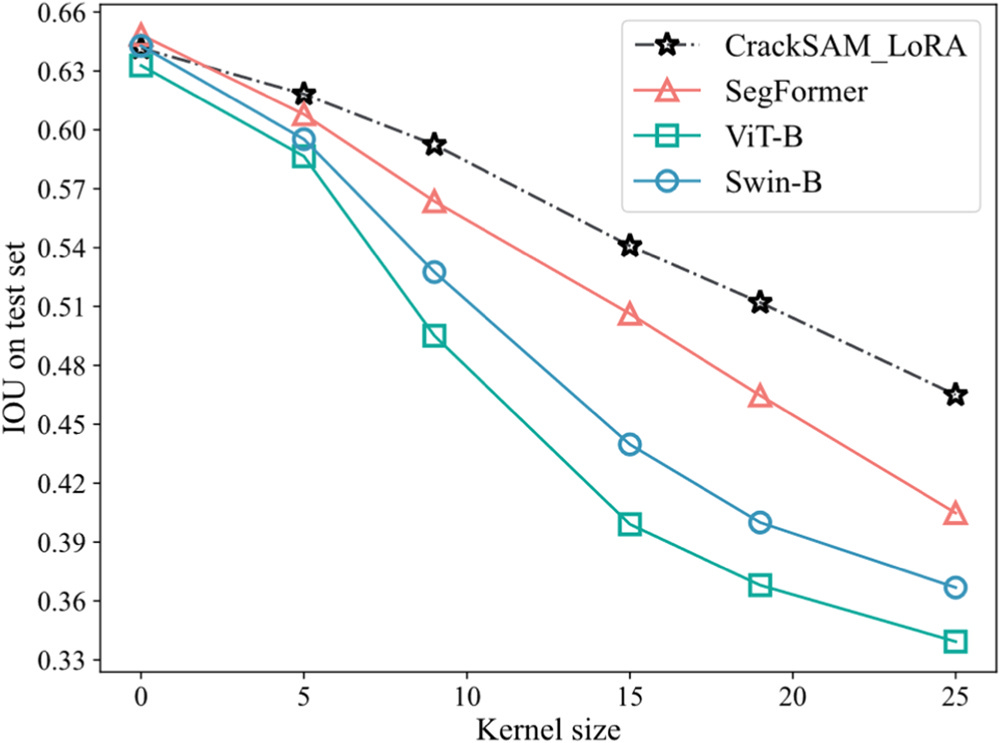
\includegraphics[width=0.98\linewidth,height=0.57\textheight,keepaspectratio]{cracksam_noise_curve.jpg}
      \par\vspace{2pt}
      {\scriptsize Le modèle publié conserve mieux son IoU quand le flou augmente.}
    \end{column}
  \end{columns}
  \source{Ge et al., \href{https://arxiv.org/abs/2312.04233}{\emph{Fine-tuning vision foundation model for crack segmentation}}, 2023. Courbe reproduite depuis l'article archivé dans le dépôt.}
\end{frame}

\begin{frame}{Notre CrackSAM 2 est une baseline utile, pas une reproduction exacte}
  \begin{columns}[T,onlytextwidth]
    \begin{column}{0.44\textwidth}
      \begin{tikzpicture}[node distance=0.22cm]
        \node[rounded corners=4pt,draw=inkblue!45,fill=softblue,
          text width=4.75cm,align=left,inner sep=6pt] (published) {
          \textbf{CrackSAM publié}\\
          {\scriptsize SAM 1 ViT-H ; LoRA/adapter ; prompt encoder et décodeur adaptés ; 2 classes}};
        \node[rounded corners=4pt,draw=warning!45,fill=warning!7,
          text width=4.75cm,align=left,inner sep=6pt,below=of published] {
          \textbf{Port local}\\
          {\scriptsize SAM 2 Hiera-L ; LoRA $q/v$ + attentions du décodeur ; 1 logit ; prétraitement différent}};
      \end{tikzpicture}
      \vspace{0.3cm}
      \begin{alertblock}{Conséquence}
        L'écart Road420 ne peut pas être attribué au seul passage de SAM à SAM 2.
      \end{alertblock}
    \end{column}
    \begin{column}{0.53\textwidth}
      \centering
      {\scriptsize IoU moyenne sur les six conditions}\par\vspace{0.15cm}
      \metriccard{inkblue}{CrackSAM publié\,/\,SAM 1}{0,5780}{référence externe}\\[0.15cm]
      \metriccard{success}{Baseline locale\,/\,SAM 2}{0,5675}{référence des ablations}\\[0.15cm]
      \metriccard{failure}{Prompt Frangi dense}{0,5563}{$-0,0112$ vs baseline}
    \end{column}
  \end{columns}
  \source{Résultats versionnés : \texttt{docs/02\_BASELINE\_COMPARISON.md}. Les protocoles/backbones diffèrent : seule la comparaison locale baseline vs Frangi est appariée.}
\end{frame}

% -----------------------------------------------------------------------------
\section{Frangi-similarité : signal utile, mauvais langage}
\frame{\sectionpage}

\begin{frame}{Frangi-graphe propose une géométrie explicite}
  \centering
  \begin{tikzpicture}[>=Latex]
    \node (rgb) {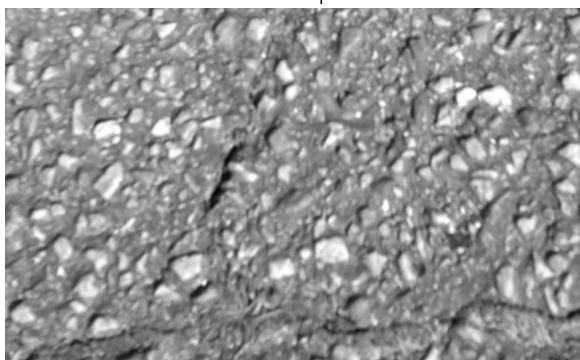
\includegraphics[width=0.29\textwidth,height=0.52\textheight,keepaspectratio]{find_visible.png}};
    \node[right=0.65cm of rgb] (sim) {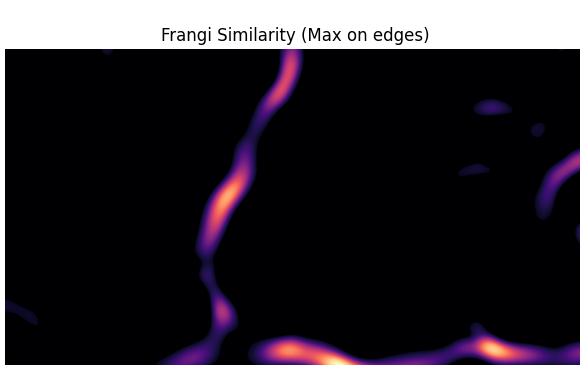
\includegraphics[width=0.29\textwidth,height=0.52\textheight,keepaspectratio]{find_similarity.png}};
    \node[right=0.65cm of sim] (graph) {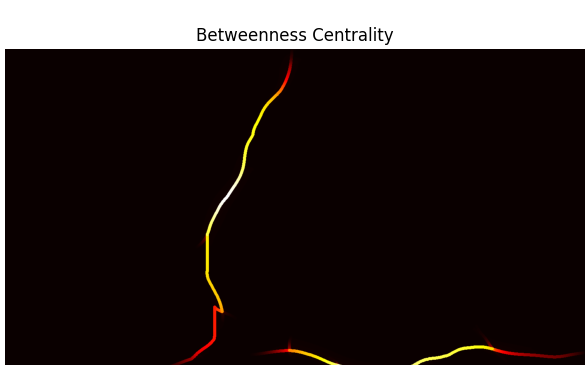
\includegraphics[width=0.29\textwidth,height=0.52\textheight,keepaspectratio]{find_centrality.png}};
    \draw[->,very thick,inkblue] (rgb) -- (sim);
    \draw[->,very thick,warning] (sim) -- (graph);
    \node[above=0.12cm of rgb,font=\bfseries] {Image visible};
    \node[above=0.12cm of sim,font=\bfseries] {Similarité Hessienne};
    \node[above=0.12cm of graph,font=\bfseries] {Chemins / centralité};
  \end{tikzpicture}

  \vspace{0.25cm}
  \begin{block}{Information potentielle}
    \centering\small Orientation, échelle, continuité et importance topologique -- mais aucune de ces grandeurs ne dit encore \og fissure\fg{}.
  \end{block}
  \source{Exemple VT-GraF, fissure 2, repris de la présentation Inria--Cerema du 10 juillet 2026.}
\end{frame}

\begin{frame}{Tentative 1 : utiliser Frangi comme un masque dense}
  \centering
  \begin{tikzpicture}[>=Latex,node distance=0.65cm]
    \node[rounded corners=5pt,draw=inkblue!50,fill=softblue,
      minimum width=2.55cm,minimum height=1.35cm,align=center] (s) {
      {\bfseries Similarité} $S(x)$\\{\scriptsize normalisée par image}};
    \node[rounded corners=5pt,draw=warning!55,fill=warning!8,
      minimum width=2.6cm,minimum height=1.35cm,align=center,right=of s] (logit) {
      $\displaystyle \log\frac{S+\varepsilon}{1-S+\varepsilon}$\\{\scriptsize pseudo-logits $256^2$}};
    \node[rounded corners=5pt,draw=failure!55,fill=softred,
      minimum width=2.85cm,minimum height=1.35cm,align=center,right=of logit] (mask) {
      {\bfseries \texttt{mask\_input}}\\{\scriptsize toujours présent dans SAM 2}};
    \draw[->,very thick] (s) -- (logit);
    \draw[->,very thick] (logit) -- (mask);

    \node[below=0.75cm of s,rounded corners=4pt,draw=failure!35,fill=softred,
      text width=3.0cm,align=center,inner sep=5pt] {\scriptsize Un faible maximum de bruit devient une réponse forte.};
    \node[below=0.75cm of logit,rounded corners=4pt,draw=failure!35,fill=softred,
      text width=3.0cm,align=center,inner sep=5pt] {\scriptsize $S\simeq0 \Rightarrow$ logit $\simeq-11{,}5$ : \og fond certain\fg{}.};
    \node[below=0.75cm of mask,rounded corners=4pt,draw=failure!35,fill=softred,
      text width=3.0cm,align=center,inner sep=5pt] {\scriptsize Une hypothèse géométrique devient une segmentation imposée.};
  \end{tikzpicture}

  \vspace{0.35cm}
  \statusbadge{failure}{Réalisé : entraînement séparé baseline / Frangi jusqu'à 70 époques}
  \source{Pipeline historique documenté dans \texttt{docs/01\_EXPERIMENTAL\_QUESTION.md} et audité par la matrice causale du 20 juillet 2026.}
\end{frame}

\begin{frame}{Ablation causale : SAM lit la géométrie, mais le prompt est mal posé}
  \begin{columns}[T,onlytextwidth]
    \begin{column}{0.58\textwidth}
      \centering
      \begin{tikzpicture}[x=5.0cm,y=0.83cm]
        \draw[->] (-0.18,0) -- (0.41,0) node[right,font=\scriptsize] {$\Delta\IoU$ macro};
        \draw[dashed,black!35] (0,-0.3) -- (0,4.25);
        \fill[failure!78] (0,3.30) rectangle (-0.0979,3.80);
        \node[anchor=east,font=\scriptsize] at (-0.16,3.55) {Frangi correct vs aucun};
        \node[anchor=west,font=\scriptsize\bfseries,text=failure] at (0.31,3.55) {$-0{,}0979$};
        \fill[success!78] (0,2.30) rectangle (0.2473,2.80);
        \node[anchor=east,font=\scriptsize] at (-0.16,2.55) {correct vs permuté};
        \node[anchor=west,font=\scriptsize\bfseries,text=success] at (0.31,2.55) {$+0{,}2473$};
        \fill[success!78] (0,1.30) rectangle (0.2700,1.80);
        \node[anchor=east,font=\scriptsize] at (-0.16,1.55) {correct vs décalé};
        \node[anchor=west,font=\scriptsize\bfseries,text=success] at (0.31,1.55) {$+0{,}2700$};
        \fill[failure!78] (0,0.30) rectangle (-0.0122,0.80);
        \node[anchor=east,font=\scriptsize] at (-0.16,0.55) {système entraîné vs baseline};
        \node[anchor=west,font=\scriptsize\bfseries,text=failure] at (0.31,0.55) {$-0{,}0122$};
        \foreach \x in {-0.1,0.1,0.2,0.3}{
          \draw (\x,0.06)--(\x,-0.06) node[below,font=\tiny] {\pgfmathprintnumber[fixed,precision=1]{\x}};
        }
      \end{tikzpicture}
    \end{column}
    \begin{column}{0.39\textwidth}
      \vspace{0.15cm}
      \begin{block}{Lecture}
        \begin{itemize}
          \item Le bon alignement apporte bien une information.
          \item Mais l'injection dense dégrade immédiatement la baseline.
          \item Après coadaptation, le gain propre du prompt reste minime.
        \end{itemize}
      \end{block}
      \begin{alertblock}{Décision}
        Abandonner \texttt{mask\_input} pour Frangi.
      \end{alertblock}
    \end{column}
  \end{columns}
  \source{Matrice causale : 8 895 images, bootstrap groupé, macro sur quatre familles. \texttt{results/causal\_prompt\_matrix\_2026-07-20}.}
\end{frame}

\begin{frame}{Sous les ombres, fissure et faux signal coexistent}
  \centering
  \imagepanel{Entrée}{shadow_gain_input.jpg}\hfill
  \imagepanel{Vérité terrain}{shadow_gain_gt.jpg}\hfill
  \imagepanel{Frangi}{shadow_gain_frangi.jpg}\hfill
  \imagepanel{Baseline}{shadow_gain_baseline.jpg}\hfill
  \imagepanel{Avec prompt}{shadow_gain_guided.jpg}

  \vspace{0.28cm}
  \begin{columns}[T,onlytextwidth]
    \begin{column}{0.61\textwidth}
      \begin{alertblock}{Même image, deux explications géométriques}
        \small Frangi répond à la fissure horizontale \textbf{et} aux trois bandes d'ombre verticales. Une décision globale ne peut pas séparer ces zones.
      \end{alertblock}
    \end{column}
    \begin{column}{0.36\textwidth}
      \centering
      \metriccard{success}{IoU baseline $\rightarrow$ prompt}{0,190 $\rightarrow$ 0,685}{gain spectaculaire, mais cas isolé}
    \end{column}
  \end{columns}
  \source{Road420, \texttt{IMG\_6353}. Le succès de ce cas ne démontre pas une robustesse générale aux ombres.}
\end{frame}

\begin{frame}{Un bon détecteur géométrique peut produire un mauvais prompt}
  \centering
  \imagepanel{Entrée}{good_detector_bad_prompt_input.jpg}\hfill
  \imagepanel{Vérité terrain}{good_detector_bad_prompt_gt.jpg}\hfill
  \imagepanel{Frangi}{good_detector_bad_prompt_frangi.jpg}\hfill
  \imagepanel{Baseline}{good_detector_bad_prompt_baseline.jpg}\hfill
  \imagepanel{Avec prompt}{good_detector_bad_prompt_guided.jpg}

  \vspace{0.3cm}
  \begin{columns}[T,onlytextwidth]
    \begin{column}{0.59\textwidth}
      \begin{block}{Diagnostic}
        \small La carte Frangi suit visuellement la fissure, mais \texttt{mask\_input} fait presque disparaître la prédiction. L'échec vient ici de l'\textbf{encodage / usage du prompt}, pas d'une absence de signal.
      \end{block}
    \end{column}
    \begin{column}{0.38\textwidth}
      \centering
      \metriccard{failure}{IoU baseline $\rightarrow$ prompt}{0,720 $\rightarrow$ 0,040}{$\Delta=-0,680$}
    \end{column}
  \end{columns}
  \source{Road420, \texttt{IMG\_6033}. Analyse de chrominance : AP2 luminance $=0,800$ malgré l'effondrement de la sortie SAM 2.}
\end{frame}

\begin{frame}{Le problème est une longue queue de pertes, pas un manque de beaux exemples}
  \centering
  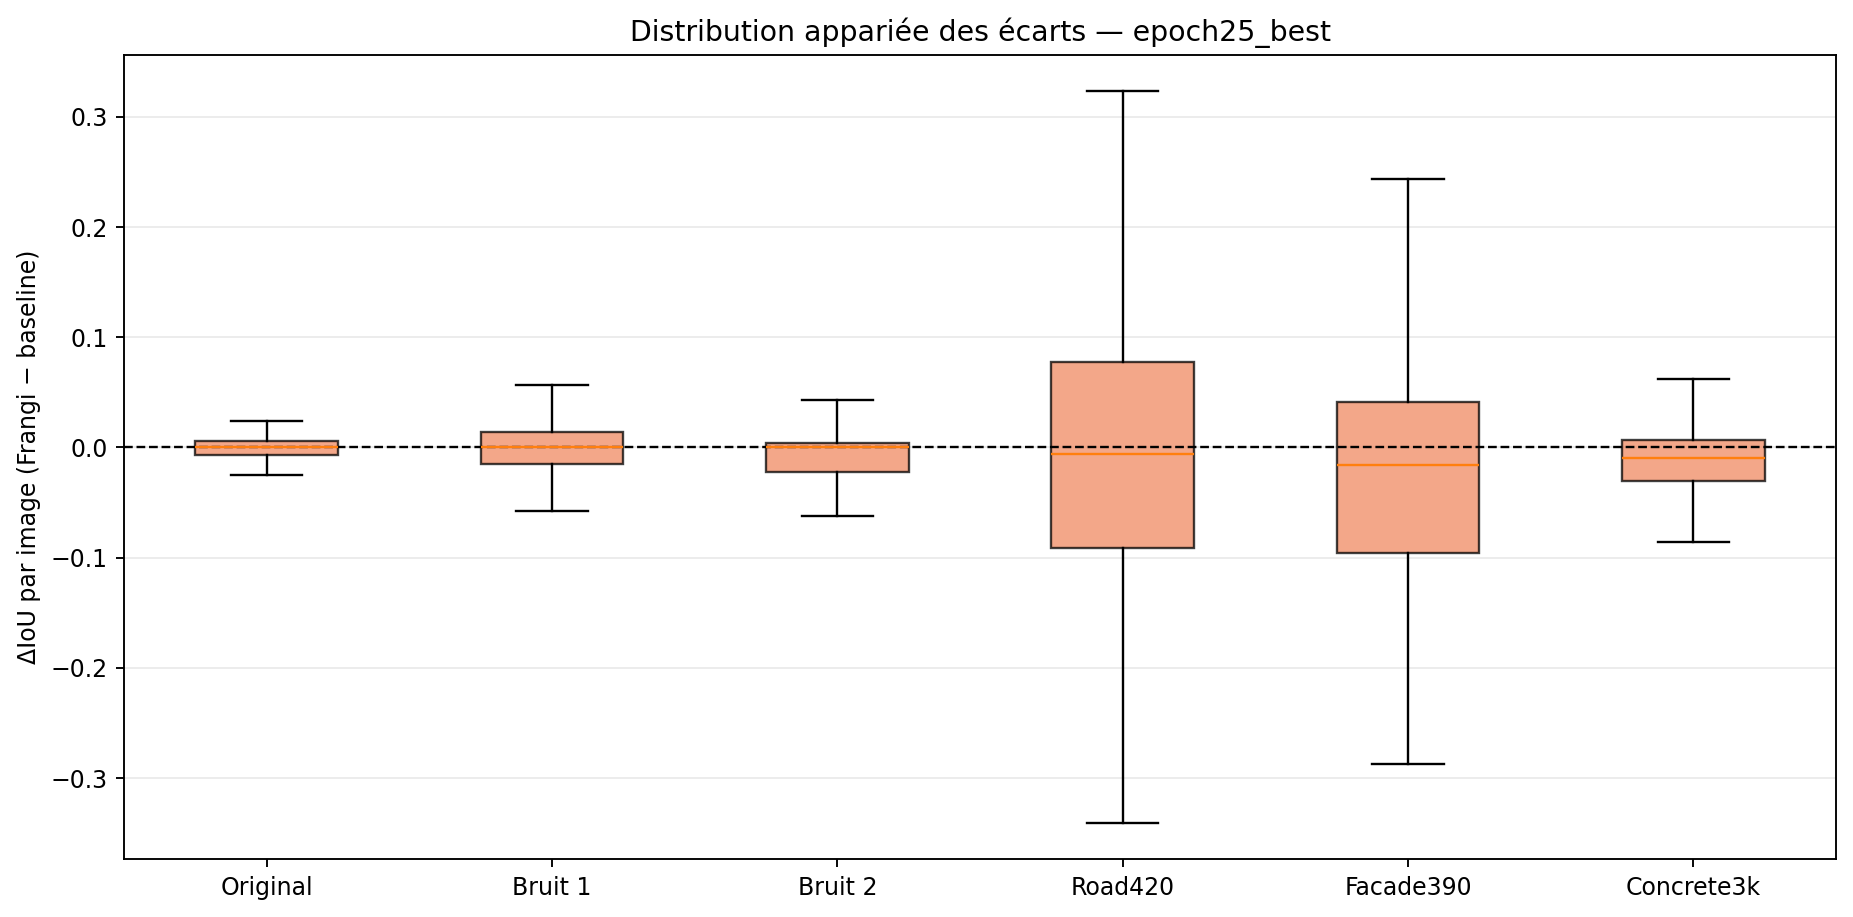
\includegraphics[width=0.88\linewidth,height=0.64\textheight,keepaspectratio]{paired_delta_iou_distributions.png}
  \begin{tikzpicture}[remember picture,overlay]
    \node[rounded corners=4pt,draw=failure!45,fill=white,align=center,
      text width=3.0cm,inner sep=5pt] at ($(current page.south east)+(-2.85cm,1.55cm)$) {
      {\scriptsize\bfseries Meilleur historique}\\[-1pt]
      {\small macro $0,5563$ vs $0,5675$}\\[-1pt]
      {\tiny Road420 : $-0,0135$ ; bruit 2 : $-0,0292$}
    };
  \end{tikzpicture}
  \source{Époque 25 sélectionnée sur validation. Les boîtes montrent les deltas IoU par image, Frangi moins baseline.}
\end{frame}

% -----------------------------------------------------------------------------
\section{Reformuler l'intégration}
\frame{\sectionpage}

\begin{frame}{Tentative 2 : corriger la baseline, puis savoir s'abstenir}
  \centering
  \begin{tikzpicture}[>=Latex,node distance=0.45cm and 0.6cm]
    \node[rounded corners=5pt,draw=inkblue!55,fill=softblue,
      minimum width=2.55cm,minimum height=1.35cm,align=center] (base) {
      {\bfseries Baseline gelée}\\$z_0$, features Hiera};
    \node[rounded corners=5pt,draw=warning!55,fill=warning!8,
      minimum width=2.65cm,minimum height=1.35cm,align=center,right=of base] (res) {
      {\bfseries Correcteur léger}\\Frangi $\rightarrow \widehat{\Delta z}$};
    \node[rounded corners=5pt,draw=success!55,fill=softgreen,
      minimum width=2.65cm,minimum height=1.35cm,align=center,right=of res] (candidate) {
      {\bfseries Candidat}\\$z_1=z_0+\widehat{\Delta z}$};
    \node[diamond,aspect=1.7,draw=black!45,fill=softgray,
      align=center,right=0.7cm of candidate] (gate) {porte\\$q$};
    \node[rounded corners=4pt,draw=success!55,fill=softgreen,
      align=center,above right=0.15cm and 0.62cm of gate] (accept) {$z_1$};
    \node[rounded corners=4pt,draw=inkblue!55,fill=softblue,
      align=center,below right=0.15cm and 0.62cm of gate] (reject) {$z_0$ exact};
    \draw[->,very thick] (base) -- (res);
    \draw[->,very thick] (res) -- (candidate);
    \draw[->,very thick] (candidate) -- (gate);
    \draw[->,thick,success] (gate) -- node[above,sloped,font=\tiny]{accepter} (accept);
    \draw[->,thick,inkblue] (gate) -- node[below,sloped,font=\tiny]{refuser} (reject);
  \end{tikzpicture}

  \vspace{0.35cm}
  \metriccard{success}{Résidu toujours ouvert}{+0,00503}{IC95 $[+0,00434;+0,00568]$}
  \hspace{0.15cm}
  \metriccard{warning}{Oracle image}{+0,00787}{plafond observé}
  \hspace{0.15cm}
  \metriccard{inkblue}{Avec porte globale}{+0,00257}{IC95 $[+0,00194;+0,00320]$}

  \source{Pilote exploratoire 3 époques : 9 121 crops / 1 727 images physiques, prédictions résiduelles OOF. Baseline non cross-fittée ; aucun benchmark externe ni test d'ombre apparié.}
\end{frame}

\begin{frame}{Version active : vérifier localement avant de corriger}
  \begin{columns}[T,onlytextwidth]
    \begin{column}{0.51\textwidth}
      \centering
      \begin{tikzpicture}[x=0.52cm,y=0.58cm,>=Latex]
        \draw[->] (0,0)--(8.2,0) node[right,font=\tiny]{profil normal à la ligne};
        \draw[->] (0,0)--(0,4.4) node[above,font=\tiny]{luminance};
        \draw[very thick,success,smooth] plot coordinates {(0.3,3.6)(1.3,3.5)(2.3,3.2)(3.1,1.1)(4.0,3.0)(5.0,3.5)(6.2,3.55)};
        \node[text=success,font=\scriptsize\bfseries] at (3.15,0.55) {vallée bilatérale};
        \draw[very thick,failure,smooth,dashed] plot coordinates {(0.3,3.3)(1.5,3.25)(2.5,3.2)(3.4,3.1)(4.0,1.3)(5.1,1.25)(6.2,1.2)};
        \node[text=failure,font=\scriptsize\bfseries] at (5.25,0.55) {marche d'ombre};
        \draw[dotted,black!45] (3.35,0)--(3.35,4.0);
      \end{tikzpicture}
      \vspace{0.15cm}
      \begin{block}{Score local $a_\theta(x)$}
        \centering\small Frangi + orientation + profil de luminance + Hiera + $z_0$.
      \end{block}
    \end{column}
    \begin{column}{0.46\textwidth}
      \begin{align*}
        z_1(x)&=z_0(x)+B(a_\theta)(x)\,\widehat{\Delta z}(x)\\[-2pt]
        B=0&\quad\Longrightarrow\quad z_1=z_0\;\text{bit à bit}
      \end{align*}
      \statusbadge{warning}{Implémenté, pas encore évalué sur GPU}
      \vspace{0.1cm}
      \begin{itemize}
        \item décision locale dans une même image ;
        \item repli exact hors bande et sous \texttt{no\_evidence} ;
        \item tests CPU : vallée/marche, pénombre, orientation.
      \end{itemize}
      \begin{alertblock}{À démontrer}
        Distingue-t-il fissures et ombres à couverture comparable ?
      \end{alertblock}
    \end{column}
  \end{columns}
  \source{Prototype \texttt{verified\_local\_v1}, décrit dans \texttt{docs/07\_SELECTIVE\_FRANGI\_EVIDENCE.md}.}
\end{frame}

% -----------------------------------------------------------------------------
\section{Ce que suggère la littérature}
\frame{\sectionpage}

\begin{frame}{Cinq idées directement transférables}
  \centering
  \litcard{failure}{SACM}{CVPR 2026}{Adaptateurs internes + externes, fusion multi-couche et raffinement en deux temps pour structures curvilignes.}
  \hspace{0.18cm}
  \litcard{inkblue}{HQ-SAM}{2023}{Fusion de features précoces/finales et jeton de sortie dédié aux détails fins.}\\[0.18cm]
  \litcard{warning}{SAM-Road}{2024}{Les embeddings SAM vérifient les arêtes avec un petit Transformer de graphe.}
  \hspace{0.18cm}
  \litcard{success}{SAC + topologie}{2024--25}{Normalisations seules pour l'adaptation ; clDice ou Skeleton Recall pour la connectivité.}\\[0.18cm]
  \litcard{inria-2024-violet}{SAM 3}{ICLR 2026}{Texte + exemplaires + tête de présence : vérificateur sémantique possible, pas remède automatique à la résolution.}

  \source{Zhu et al. (SACM), Ke et al. (HQ-SAM), Hetang et al. (SAM-Road), Rostami et al. (Segment Any Crack), Shit et al. (clDice), Kirchhoff et al. (Skeleton Recall), Carion et al. (SAM 3).}
\end{frame}

\begin{frame}{Feuille de route proposée : une hypothèse à la fois}
  \centering
  \begin{tikzpicture}[>=Latex,node distance=0.18cm]
    \node[rounded corners=5pt,draw=inkblue!50,fill=softblue,
      text width=10.6cm,minimum height=0.85cm,align=left,inner sep=6pt] (p0) {
      \textbf{0. Baseline fidèle} \quad SAM 2.1 ; LoRA Hiera + décodeur/prompt encoder ; ablation normalisations.};
    \node[rounded corners=5pt,draw=success!50,fill=softgreen,
      text width=10.6cm,minimum height=0.85cm,align=left,inner sep=6pt,below=of p0] (p1) {
      \textbf{1. Raster sélectif} \quad 5 folds OOF ; vrai Frangi vs absence/décalé/permuté ; validation \href{https://www.ieee-jas.net/article/doi/10.1109/JAS.2023.123447}{Shadow-Crack}.};
    \node[rounded corners=5pt,draw=warning!50,fill=warning!8,
      text width=10.6cm,minimum height=0.85cm,align=left,inner sep=6pt,below=of p1] (p2) {
      \textbf{2. Graphe explicite} \quad vérifier noeuds/arêtes/composantes avec features Hiera ; comparer au raster à capacité égale.};
    \node[rounded corners=5pt,draw=inria-2024-violet!50,fill=inria-2024-violet!7,
      text width=10.6cm,minimum height=0.85cm,align=left,inner sep=6pt,below=of p2] (p3) {
      \textbf{3. Pilote SAM 3} \quad texte \texttt{fissure} + exemplaires positifs/négatifs ; même protocole, sans migration prématurée.};
    \draw[->,thick] (p0) -- (p1);
    \draw[->,thick] (p1) -- (p2);
    \draw[->,thick] (p2) -- (p3);
  \end{tikzpicture}

  \vspace{0.18cm}
  \begin{block}{Critères à pré-enregistrer}
    \centering\scriptsize
    $\Delta\IoU_{macro}\geq +0{,}005$ et borne IC95 $>0$
    \quad $\vert$ \quad faux signal ombre $-20\%$
    \quad $\vert$ \quad rappel squelette : perte $\leq5$ points
    \quad $\vert$ \quad pertes $<-0{,}05$ divisées par 2
  \end{block}
\end{frame}

\begin{frame}{Conclusion : Frangi ne doit pas être le masque}
  \centering
  \begin{tikzpicture}[>=Latex,node distance=0.65cm]
    \node[rounded corners=6pt,draw=failure!55,fill=softred,
      minimum width=3.6cm,minimum height=1.65cm,align=center] (bad) {
      {\Large\bfseries\color{failure} À abandonner}\\[2pt]
      Frangi $\rightarrow$ \texttt{mask\_input}\\
      {\scriptsize dense, toujours actif}};
    \node[rounded corners=6pt,draw=success!55,fill=softgreen,
      minimum width=5.3cm,minimum height=1.65cm,align=center,right=of bad] (good) {
      {\Large\bfseries\color{success} À tester proprement}\\[2pt]
      proposer $\rightarrow$ vérifier localement $\rightarrow$ corriger\\
      {\scriptsize avec fallback exact et porte calibrée}};
    \draw[->,very thick,black!50] (bad) -- (good);
  \end{tikzpicture}

  \vspace{0.55cm}
  \begin{columns}[T,onlytextwidth]
    \begin{column}{0.32\textwidth}
      \centering
      \textbf{Acquis}\\[2pt]
      {\small la géométrie Frangi est lue, mais l'interface dense est nuisible}
    \end{column}
    \begin{column}{0.32\textwidth}
      \centering
      \textbf{Prochaine preuve}\\[2pt]
      {\small \texttt{verified\_local\_v1}, 5 folds et ombres appariées}
    \end{column}
    \begin{column}{0.32\textwidth}
      \centering
      \textbf{Option}\\[2pt]
      {\small SAM 3 comme vérificateur par concept/exemplaire}
    \end{column}
  \end{columns}
  \source{Conclusion limitée aux résultats disponibles au 25 juillet 2026.}
\end{frame}

\appendix

\begin{frame}{Références essentielles}
  \scriptsize
  \begin{columns}[T,onlytextwidth]
    \begin{column}{0.49\textwidth}
      \begin{itemize}
        \item Kirillov et al., \href{https://arxiv.org/abs/2304.02643}{\emph{Segment Anything}}, ICCV 2023.
        \item Ravi et al., \href{https://arxiv.org/abs/2408.00714}{\emph{SAM 2: Segment Anything in Images and Videos}}, 2024.
        \item Carion et al., \href{https://arxiv.org/abs/2511.16719}{\emph{SAM 3: Segment Anything with Concepts}}, ICLR 2026.
        \item Ge et al., \href{https://arxiv.org/abs/2312.04233}{\emph{Fine-tuning vision foundation model for crack segmentation}}, 2023.
        \item Rostami et al., \href{https://arxiv.org/abs/2504.14138}{\emph{Segment Any Crack}}, 2025.
        \item Zhu et al., \href{https://openaccess.thecvf.com/content/CVPR2026/html/Zhu_Dual-level_Adapter_Boosting_Prompt-free_Curvilinear_Structure_Segmentation_CVPR_2026_paper.html}{\emph{Dual-level Adapter Boosting Prompt-free Curvilinear Structure Segmentation}}, CVPR 2026.
      \end{itemize}
    \end{column}
    \begin{column}{0.49\textwidth}
      \begin{itemize}
        \item Ke et al., \href{https://arxiv.org/abs/2306.01567}{\emph{Segment Anything in High Quality}}, 2023.
        \item Hetang et al., \href{https://arxiv.org/abs/2403.16051}{\emph{Segment Anything Model for Road Network Graph Extraction}}, 2024.
        \item Shit et al., \href{https://arxiv.org/abs/2003.07311}{\emph{clDice}}, 2020/2021.
        \item Kirchhoff et al., \href{https://arxiv.org/abs/2404.03010}{\emph{Skeleton Recall Loss}}, 2024.
        \item Fan et al., \href{https://www.ieee-jas.net/article/doi/10.1109/JAS.2023.123447}{\emph{Pavement Cracks Coupled With Shadows}}, IEEE/CAA JAS 2023.
        \item Frangi et al., \emph{Multiscale Vessel Enhancement Filtering}, MICCAI 1998.
      \end{itemize}
    \end{column}
  \end{columns}
  \vspace{0.25cm}
  \begin{block}{Traçabilité interne}
    \tiny Résultats historiques : \texttt{results/frangi\_milestone\_report} ; ablation causale : \texttt{results/causal\_prompt\_matrix\_2026-07-20} ; pilote résiduel : \texttt{artifacts/frangigraph\_logistic\_pilot\_e3\_seed3407} ; méthode active : \texttt{docs/07\_SELECTIVE\_FRANGI\_EVIDENCE.md}.
  \end{block}
\end{frame}

\end{document}
